% This is text associated with the open textbook "Open Electromagnetics"
% See immediately below for author, date
% This work is licensed under the Creative Commons Attribution-ShareAlike 4.0 International License. (CC BY-SA 4.0) 
% To view a copy of the license, visit http://creativecommons.org/licenses/by-sa/4.0/

%ORB TITLE Parallel Plate Waveguide: Introduction
%ORB AUTHOR 0        # S.W. Ellingson, Virginia Tech (ellingson@vt.edu)
%ORB DATE 20191121   # yyyymmdd
%ORB ABSTRACT 

\label{m0173_Parallel_Plate_Waveguide_Introduction} % <-- Must match name of this file and module directory name.  Don't mess with this!
\index{waveguide!parallel plate|(}
\index{parallel-plate waveguide|see{waveguide}}

A parallel plate waveguide is a device for guiding the propagation of waves between two perfectly-conducting plates.
Our primary interest in this structure is as a rudimentary model applicable to a broad range of engineering problems.
Examples of such problems include analysis of the fields within microstrip line and propagation of radio waves in the ionosphere.

Figure~\ref{m0173_fParallelPlateWaveguide} shows the geometry of interest.
Here the plates are located at $z=0$ and $z=a$. %; therefore the distance between the plates is $a$.
The plates are assumed to be infinite in extent, and therefore there is no need to consider fields in the regions $z<0$ or $z>a$.
For this analysis, the region between the plates is assumed to consist of an ideal (lossless) material exhibiting real-valued permeability $\mu$ and real-valued permittivity $\epsilon$.
%
\begin{figure}[b!] % <--- "[b]" for first figure in section *only*; delete for 2nd and subsequent figures
\begin{center}
\pdftooltip{{  % note double braces
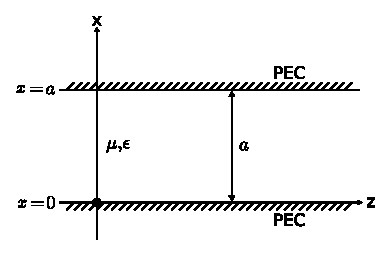
\includegraphics[width=0.8\columnwidth]{modules/m0173_fParallelPlateWaveguide.eps} 
% https://commons.wikimedia.org/wiki/File:Geometry_for_analysis_of_fields_in_parallel_plate_waveguide.svg
}}{For a z-x Cartesian coordinate system two parallel plates are a distance small a apart. The interior region is labeled small mu comma small epsilon.}
\end{center}
\centerline{\scriptsize 
\copyright~\hyperref[m0173_fParallelPlateWaveguide_Credit]{C.\ Wang} 
\href{https://creativecommons.org/licenses/by-sa/4.0/}{CC BY-SA 4.0} (modified)
} % \centerline 
\caption{
\label{m0173_fParallelPlateWaveguide}
Geometry for analysis of fields in a parallel plate waveguide.
}
\end{figure}

Let us limit our attention to a region within the waveguide which is free of sources.
Expressed in phasor form, the electric field intensity is governed by the wave equation
%
\begin{equation}
\nabla^2 \widetilde{\bf E} + \beta^2 \widetilde{\bf E} = 0
\label{m0173_eWE}
\end{equation} 
%
where
%
\begin{equation}
\beta = \omega \sqrt{\mu \epsilon}
\end{equation}
%
Equation~\ref{m0173_eWE} is a partial differential equation.
This equation, combined with boundary conditions imposed by the perfectly-conducting plates, is sufficient to determine a unique solution.
This is most easily done in Cartesian coordinates, as we shall now demonstrate.
First we express $\widetilde{\bf E}$ in Cartesian coordinates:
%
\begin{equation}
\widetilde{\bf E} = \hat{\bf x}\widetilde{E}_x + \hat{\bf y}\widetilde{E}_y + \hat{\bf z}\widetilde{E}_z
\label{m0173_eE}
\end{equation}
%
This facilitates the decomposition of Equation~\ref{m0173_eWE} into separate equations governing the $\hat{\bf x}$, $\hat{\bf y}$, $\hat{\bf z}$ components of $\widetilde{\bf E}$:
%
\begin{flalign}
\nabla^2 \widetilde{E}_x + \beta^2 \widetilde{E}_x &= 0 \\
\nabla^2 \widetilde{E}_y + \beta^2 \widetilde{E}_y &= 0 \\
\nabla^2 \widetilde{E}_z + \beta^2 \widetilde{E}_z &= 0 
\end{flalign} 

Next we observe that the operator $\nabla^2$ may be expressed in Cartesian coordinates as follows:
%
\begin{equation}
\nabla^2 = \frac{\partial^2}{\partial x^2} + \frac{\partial^2}{\partial y^2} + \frac{\partial^2}{\partial z^2} 
\end{equation}
%
so the equations governing the Cartesian components of $\widetilde{\bf E}$ may be written as follows:
%
\begin{flalign}
\frac{\partial^2}{\partial x^2}\widetilde{E}_x + \frac{\partial^2}{\partial y^2}\widetilde{E}_x + \frac{\partial^2}{\partial z^2}\widetilde{E}_x &= - \beta^2 \widetilde{E}_x \label{m0173_eEfx} \\
\frac{\partial^2}{\partial x^2}\widetilde{E}_y + \frac{\partial^2}{\partial y^2}\widetilde{E}_y + \frac{\partial^2}{\partial z^2}\widetilde{E}_y &= - \beta^2 \widetilde{E}_y \label{m0173_eEfy} \\
\frac{\partial^2}{\partial x^2}\widetilde{E}_z + \frac{\partial^2}{\partial y^2}\widetilde{E}_z + \frac{\partial^2}{\partial z^2}\widetilde{E}_z &= - \beta^2 \widetilde{E}_z \label{m0173_eEfz} 
\end{flalign} 

Let us restrict our attention to scenarios that can be completely described in two dimensions; namely $x$ and $z$, and for which there is no variation in $y$.
This is not necessarily required, however, it is representative of a broad class of relevant problems, and allows Equations~\ref{m0173_eEfx}--\ref{m0173_eEfz} to be considerably simplified. 
If there is no variation in $y$, then partial derivatives with respect to $y$ are zero, yielding:
%
\begin{flalign}
\frac{\partial^2}{\partial x^2}\widetilde{E}_x + \frac{\partial^2}{\partial z^2}\widetilde{E}_x &= - \beta^2 \widetilde{E}_x \label{m0173_eEfx2} \\
\frac{\partial^2}{\partial x^2}\widetilde{E}_y + \frac{\partial^2}{\partial z^2}\widetilde{E}_y &= - \beta^2 \widetilde{E}_y \label{m0173_eEfy2} \\
\frac{\partial^2}{\partial x^2}\widetilde{E}_z + \frac{\partial^2}{\partial z^2}\widetilde{E}_z &= - \beta^2 \widetilde{E}_z \label{m0173_eEfz2} 
\end{flalign}

The solution to the parallel plate waveguide problem may now be summarized as follows:
The electric field $\widetilde{\bf E}$ (Equation~\ref{m0173_eE}) is the solution to simultaneous Equations~\ref{m0173_eEfx2}--\ref{m0173_eEfz2} subject to the boundary conditions that apply at the PEC surfaces at $z=0$ and $z=d$; namely, that the tangent component of $\widetilde{\bf E}$ is zero at these surfaces.

At this point, the problem has been reduced to a routine exercise in the solution of partial differential equations.
However, a somewhat more useful approach is to first decompose the total electric field into transverse electric (TE) and transverse magnetic (TM) components,\footnote{For a refresher on TE-TM decomposition, see Section~\ref{m0166_Decomposition_into_TE_and_TM}.} and determine the solutions to these components separately.
The TE component of the electric field is parallel to the plates, and therefore transverse (perpendicular) to the plane shown in Figure~\ref{m0173_fParallelPlateWaveguide}.  
Thus, the TE component has $\widetilde{E}_x=\widetilde{E}_z=0$, and only $\widetilde{E}_y$ may be non-zero.
The TM component of the magnetic field intensity ($\widetilde{\bf H}$) is parallel to the plates, and therefore transverse to the plane shown in Figure~\ref{m0173_fParallelPlateWaveguide}.  
Thus, the TM component has $\widetilde{H}_x=\widetilde{H}_z=0$, and only $\widetilde{H}_y$ may be non-zero.
As always, the total field is the sum of the TE and TM components.

The TE and TM solutions are presented in Sections~\ref{m0174_Parallel_Plate_Waveguide_TE_Electric} (Electric component of the TE solution),
\ref{m0175_Parallel_Plate_Waveguide_TE_Magnetic} (Magnetic component of the TE solution), and
\ref{m0177_Parallel_Plate_Waveguide_TM_Electric} (Electric component of the TM solution).
The magnetic component of the TM solution can be determined via a straightforward variation of the preceding three cases, and so is not presented here.

Presentation of the solution for the fields in a parallel plate waveguide under the conditions described in the section continues in Section~\ref{m0174_Parallel_Plate_Waveguide_TE_Electric}. 

\index{waveguide!parallel plate|)}


